\section{What is a Translation Memory?}

A translation memory is a tool for a computer assisted human translation.
 The core idea behind translation memories is the assumption that sentences that are similar in the source language will have probably a similar translation in the target language. Then, if the tool is able to provide the translator a translation of a similar sentence, there is a big chance the translator can just edit a little the provided sentence and get the translation he wants.

The translation memories are widely used in the translation industry, mostly while translating technical documentation and localization of software. In such cases the translators usually take advantage from that the new version of manuals of software does not differ much from the previous version. A survey \footnote{Elina Lagoudaki (2006), "Translation Memory systems: Enlightening users' perspective. Key finding of the TM Survey 2006 carried out during July and August 2006. (Imperial College London, Translation Memories Survey 2006), p.16} among companies producing multilingual documentation for their products in 2006 showed that 82.5 \% out of 874 such companies uses a TM system.

While using a translation memory there is usually an tendency to keep the database as clean as possible in terms of domain -- to contain only relevant for translated topics. The reasons to do so are effort to keep the database as small as possible not to make the database search too slow and not spoil the terminology that is used in the particular area. To keep the the terminology consistent the domain glossaries are usually used.

There are several reasons in using translation memories makes the translators' work more efficient. The main advantage is that it reduce the cost and makes the translation process faster because the amount of the translators work is lower -- the work that has been done once can be easily reused for many times. It help keeps consistency of translation between more documents and also with their previous versions. It is also quite easy to ensure that each sentence of the original document was translated into a segment of the target language document.

There also some obstacles in using the translation memory systems. The professional Translation Memory Management Systems are very expensive and the maintenance of such system can be demanding as well. From the view of the quality of the translation there is a danger that the translator could translate the text mechanically sentence by sentence instead of focusing on translating the message of the text.

In contrast to the completely machine translation it is still the human translator who controls the whole process of translation. Nevertheless, the improvements in the machine translation allows to provide a machine translation output together with the TM candidates.

\section{Usual implementation}

A simple option is to provide only candidate sentences where the sentences in the source language matches exactly each other. Usually the database is relatively sparse and probably no sentences would be retrieved. In such cases a fuzzy matching algorithm is used to retrieve similar also similar sentences where the similarity is usually a metric based on the Levensthein editing distance.

Before using the translation memory itself, some preprocessing may be necessary. Often the text extraction is needed (e.g. in case of localization of user interfaces). Sometimes finding the terminology or other named entities and always segmentation to elementary units, usually sentences, is done. This components can be either rule based or statistical. 

During the translation process the system retrieves the similar sentences from the database of already translated sentences. Usually sentences having the smallest letter based or word based \emph{Levensthein editing distance} are used.

The Levensthein distance of two strings is a minimum number of edits (insertions, deletions and substitutions) which is needed to transform one string to another. A modification called Damerau–Levenshtein distance allowing also transposition of two adjacent letters can be also used.

Originally a bottom-up dynamic programming algorithm was used -- a distance of two strings is computed from the knowledge of the of the distance of one letter shorter prefixes. Later the Bitap algorithm used in Unix tool \emph{agrep} appeared. Theoretically also a finite state machine (Levenshtein transducer) can be constructed for Levensthein distance.

\begin{figure}
\begin{center}
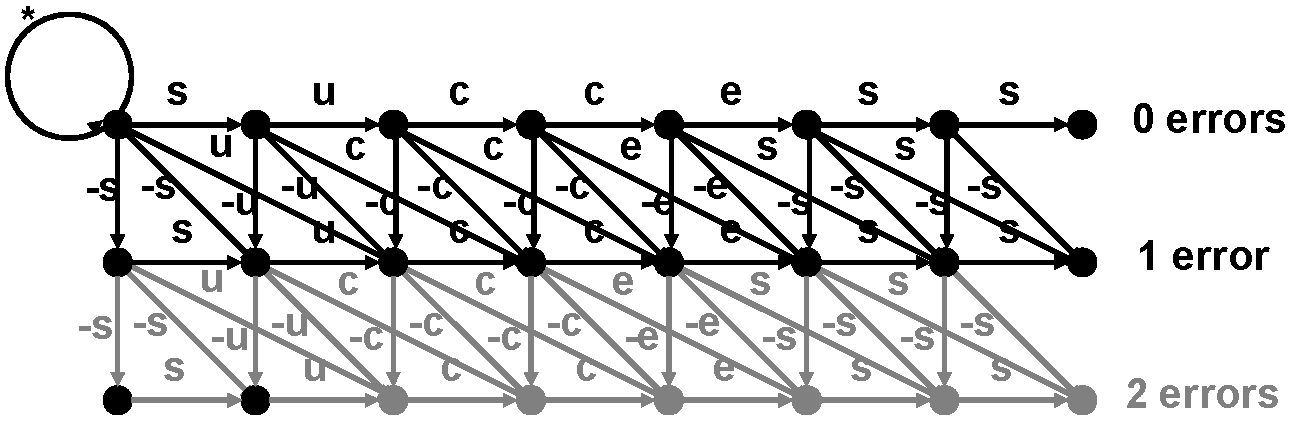
\includegraphics[scale=0.65]{./figures/levensthein.pdf}
\end{center}

\caption{An example of the Levensthein transducer for the word \emph{"success"}. (Taken from the study material for the \emph{Information Retrieval Systems} course at MFF UK by Michal Kopecký.)}
\end{figure}

For bigger databases the online algorithms begin to be very slow a preprocessing of the database is necessary. Some sophisticated indexing methods are used, among them the suffix trees or $n$-gram indexes. The candidates retrieved from such indexes are later examined more carefully.

\section{Current TM tools}

... most of professional translator use SDL Trados, some open-source projects, IBM released its own TM as open source, OmegaT widely used for localization of open source projects

... MyMemory project is somehow very similar to our project -- a big general purpose translation memory. 